This thesis continues to build on the Cellular Automata Research Platform (CARP), which is the result of three previous master theses at NTNU.
The original implementation was made by Djupdal in 2003.
It was then extended with a range of various output methods by Aamodt in 2005.
Finally, it was further extended and optimized in expectation of new hardware by Støvneng in 2014.

\TODO
Functionality.
Purpose.
\figurename~\ref{fig:overview-general}.

\begin{figure}[!ht]
    \centering
    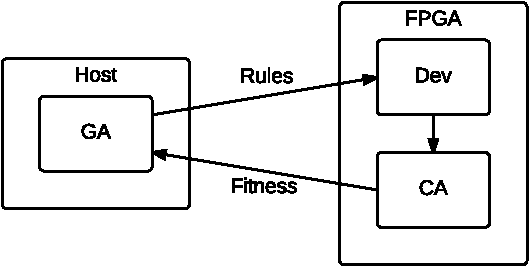
\includegraphics[width=0.57\textwidth]{figures/overview-general}
    \caption[System design]{
        High-level system design.
    }
    \label{fig:overview-general}
\end{figure}

%==============================================================================%

\section{Djupdal}

In 2002, NTNU invested in a CompactPCI computer with a NallaTech BenERA FPGA board to be used for research within the field of evolutionary hardware.
The task of developing a platform for the system, based on a matrix of sblocks, fell to Djupdal \cite{djupdal2003sblock}.

An overview of the resulting hardware platform is shown in \figurename~\ref{fig:overview-djupdal}.
It consists of the mentioned sblock matrix, block RAM (BRAM) for storing the state and type of each cell, a development unit, control logic, and a PCI communication unit.

\begin{figure}[!ht]
    \centering
    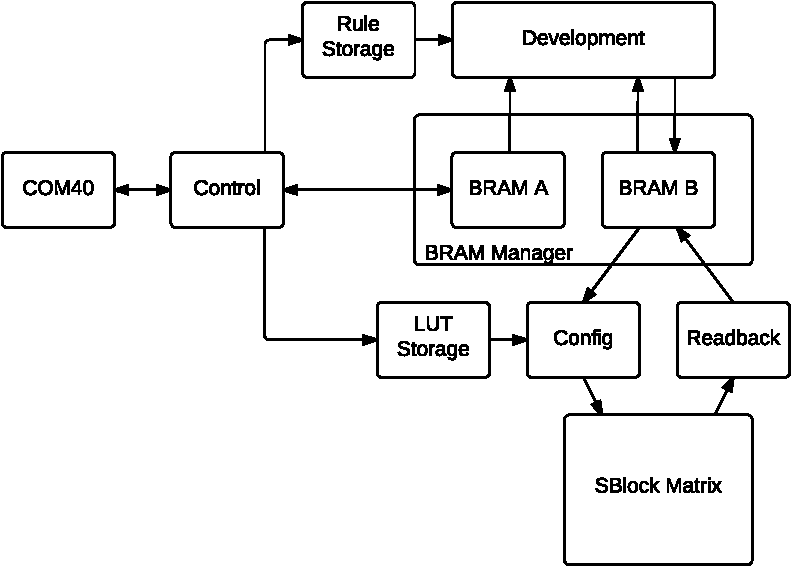
\includegraphics[width=0.86\textwidth]{figures/overview-djupdal}
    \caption[Djupdal's hardware design]{
        High-level block diagram of the hardware platform after Djupdal's original work.
    }
    \label{fig:overview-djupdal}
\end{figure}

The system is meant to be controlled by a computer running a genetic algorithm.
A common flow of operation is to initialize the system with the genotype, develop it into its phenotype, run the SBM, and send the new states back to the computer.
The computer then uses the newly received state data to calculate a fitness score.

The system is initialized by writing states and types to BRAM A, in addition to storing development rules and LUT conversion rules.
Then a development step can be performed by reading cell types from BRAM A\footnotemark, testing development rules, and writing the (possibly changed) types back to BRAM B.
\footnotetext{
    After the first 8 rules have been tested on all cells, center cell types are read from BRAM B instead.
    This is needed to prevent the result of a rule in an earlier iteration from being deleted if no rules trigger in a later iteration.
}
The development unit tests 8 rules on 2 cells each cycle in raster order.
Optionally, the BRAMs can be logically swapped and further development steps performed.
The SBM can then be configured by translating the types in BRAM B into LUT entries according to the LUT conversion rules, before being run for a desired amount of cycles.
Afterwards, the new states in the SBM can be read back into BRAM B, swapped into BRAM A, and sent to the computer.

The design is split into two clock domains; the communication unit uses 40 MHz to be able to interface with PCI, while the rest uses 80 MHz for higher performance.

%==============================================================================%

\section{Aamodt}

There was one major bottleneck in the original design.
To calculate the fitness of an individual, the state of each cell had to be transferred to the computer over the PCI interface.
Having a dedicated hardware unit would greatly improve the performance.
Additionally, it was desired to have more information about the development process.
The task of realizing this fell to Aamodt \cite{aamodt2005sblock}.

An overview of the hardware platform with Aamodt's additions is shown in \figurename~\ref{fig:overview-aamodt}.
The additions consists of a Run-Step Function (RSF) that calculates the number of live cells, BRAM to store the numbers, a fitness function, and two information outputs from the development unit.

\begin{figure}[!ht]
    \centering
    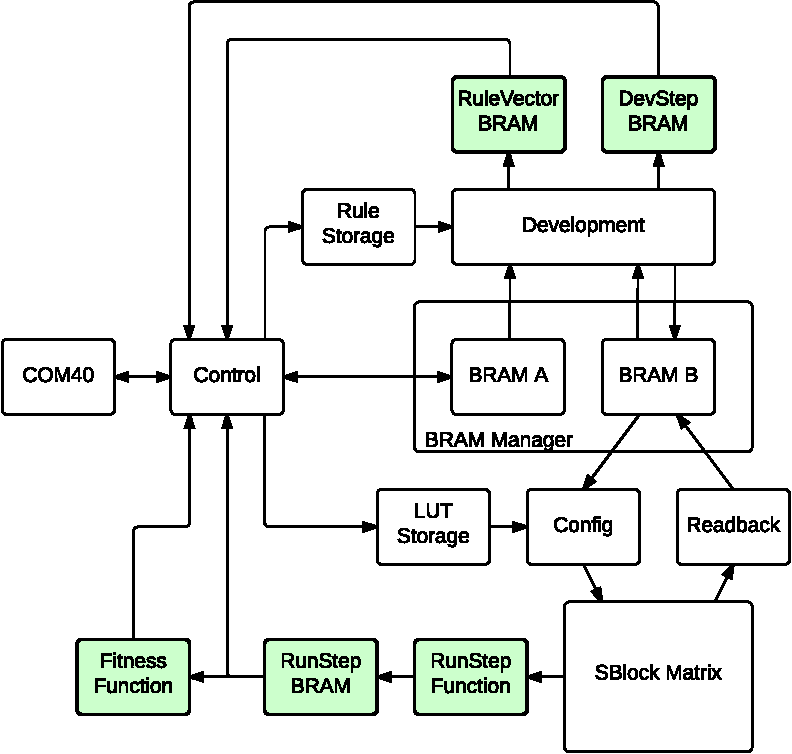
\includegraphics[width=0.86\textwidth]{figures/overview-aamodt}
    \caption[Aamodt's hardware design]{
        High-level block diagram of the hardware platform after Aamodt's work.
        Additions are highlighted in green.
    }
    \label{fig:overview-aamodt}
\end{figure}

The rule vector BRAM stores lists of which rules were triggered and not for the last 256 development steps.
The lists are implemented as bit-vectors where each bit represents the status of a rule for a single development step.
The development step BRAM is more detailed; it stores which rule was triggered for each cell.
However, it only has storage space for one development step.

The run-step function calculates the number of live cells after each SBM update by using a large adder tree.
The numbers are stored in run-step BRAM for later usage by the fitness function, which is replaceable.

%==============================================================================%

\section{Støvneng}

In expectation of receiving new hardware with a larger and faster FPGA, there was a demand to optimize the platform by taking advantage of the increased resource pool.
Extending the platform into the third dimension was also a lucrative thought, as doing so allows more complex signal pathways to form within the cellular automata.
It was also desired to have a Discrete Fourier Transform (DFT) for interpretation of the RSF data; it should give very useful data according to Berg's research \cite{berg2013ca}.
The task of realizing this was taken on by Støvneng \cite{stovneng2014sblock}.

An overview of the hardware platform with Støvneng's additions and optimizations is shown in \figurename~\ref{fig:overview-stovneng}.
The only addition is the DFT, but nearly all units has been optimized, yielding a speedup of 4 for most operations.

\begin{figure}[!ht]
    \centering
    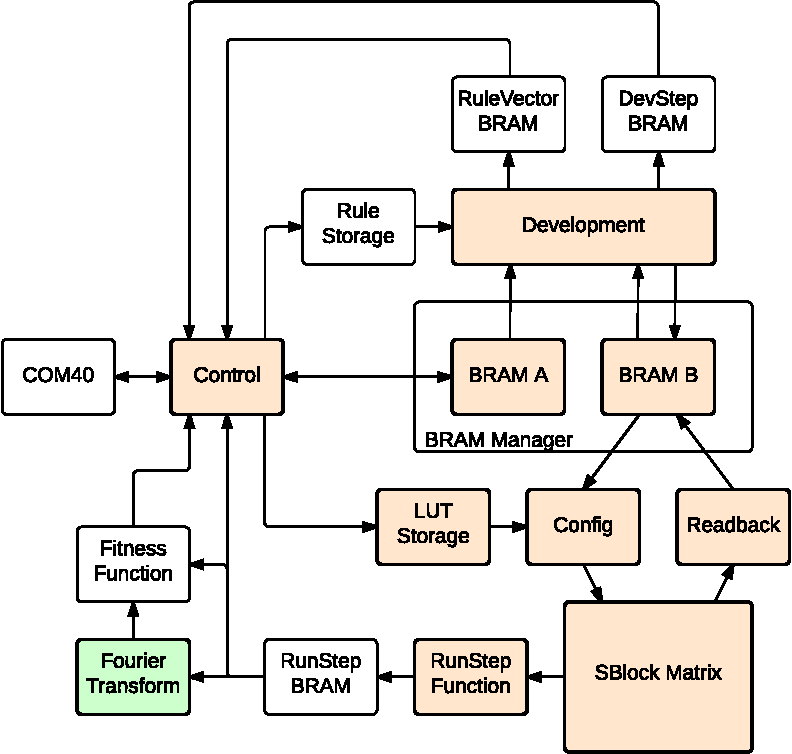
\includegraphics[width=0.86\textwidth]{figures/overview-stovneng}
    \caption[Støvneng's hardware design]{
        High-level block diagram of the hardware platform after Støvneng's work.
        Additions are highlighted in green, and optimizations and 3D modifications in orange.
    }
    \label{fig:overview-stovneng}
\end{figure}

Unfortunately, due to some challenges with manufacturing, Støvneng was unable to get hold of the new hardware for the duration of his project.
The system was therefore only verified in simulation, and the PCI communication unit was not upgraded for the PCI Express connection on the new board.

%==============================================================================%

\section{Issues}

\todo{move me maybe?}

The original idea was to complete Støvneng's design by implementing the PCI Express module and driver in the specialization project leading up to this thesis, and then proceed to use the platform for research.
However, after successful integration, verification of the platform revealed multiple serious issues, which are listed in Table~\ref{tab:issues}.
The full project report can be read in Appendix~\ref{app:specialization-project}.

\begin{table}[!ht]
    \renewcommand{\arraystretch}{1.3}
    \centering
    \begin{tabular}{l|l}
        \bfseries Type & \bfseries Issue \\
        \hline
        Severe & Many instructions fails or does not follow specification \\
        Severe & Unnecessarily complex code, making debugging nearly impossible \\
        Minor & Extensive use of outdated features (tristate buffers and global resets) \\
        Minor & Two different hardware designs and software APIs (2D and 3D) \\
        Minor & DFT twiddle factors are generated by an external python program \\
        Minor & Parameters must be set in both hardware design and software API \\
        Minor & Almost no control flow available in the hardware design \\
    \end{tabular}
    \caption[Issues]{Issues with the existing design.}
    \label{tab:issues}
\end{table}

Starting from a blank slate would allow the platform to be made more modular, more configurable, and more maintainable.
Also, it would be possible to unify the 2D and 3D designs and remove external dependencies.
This led to the decision of rebuilding the entire platform from scratch.
